\documentclass[english, a4paper]{article}
% package
\usepackage{mwe}

% Title in english
\title{Abstract title}

% Authors
\author{
Author A\affmark[1], Author B\affmark[1] and Author C\affmark[2]\\
\affaddr{\affmark[1] Affiliation of authors A and B}\\
\affaddr{\affmark[2] Affiliation of author C}
}

\begin{document}

\maketitle

The abstract of the paper may not exceed two pages. Please prepare an abstract without dividing it into chapters. You should start by providing the title of the abstract in English ("Title in English"), personal data of the speaker (Name, surname and affiliation).

The abstract of the paper should be prepared using this template or Microsoft Word version. The *.tex and *.sty, or *.docx version together with the pictures (in * .jpg or * .png format, each max. 1 MB) should be sent to the address \textbf{kme@pwr.edu.pl} by \textbf{ 01/11/2020}.

This template provides exemplary structures (equations, tables, figures, enumerations, literature). Please fill them in with your content. Unnecessary, structures can be suspended by putting \% at the beginning of the line, or deleted.

Please use drawings in *.eps, *.pdf *.jpg, *.png format. All raster figures should be of good quality (300dpi). All used images should be attached when when You will be sending abstract.

Provide literature items in accordance with the template. Please quote using e.g. $\backslash$cite\{Aref1\} which will create \cite{Aref1}. When compiling literature for the first time please do it twice so that the references to the literature are filled in. The abstract should limit the number of cited publications to the three most important ones.

Example of \textbf{enumeration} is shown below (instead of \textbf{itemize} you can use \textbf{enumerate} to number items in your list).

\begin{itemize}
\item top: 2,0 cm,
\item bottom: 2,0 cm
\item left:  3,5 cm
\item right: 2,0 cm
\end{itemize}

An example of a text excerpt with \textbf{equations} is shown below.

The equations of motion of viscous and incompressible fluid have the form (equations \ref{eom} and \ref{incmp} - equation reference has form  $\backslash$ref\{eom\}, the equation definition has additional $\backslash$label\{eom\}, which creates basis of reference) \cite{Kochin, Aref1}:
\begin{equation}\label{eom}
\frac{\partial{\mathbf{u}}}{\partial t}+(\mathbf{u} \cdot \nabla)\mathbf{u}=-\frac{1}{\rho}\nabla p+\nu \Delta \mathbf{u},
\end{equation}
\begin{equation}\label{incmp}
\nabla \cdot \mathbf{u}=0,
\end{equation}
gdzie $\mathbf{u}=(u,v,w)$ is the velocity vector, $\rho$ -- fluid density, $p$ -- pressure  and $\nu$ --  kinematic viscosity coefficient.

The following sections show examples of placing \textbf{charts, pictures and tables.}
Single graph or photo  (Fig.\ref{obraz1} - the figure reference is created the same way the equation reference is created):
\begin{figure}[h!]
\centering
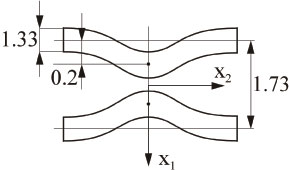
\includegraphics[width=0.35\linewidth]{figure1.jpg}
\caption{One image with caption}\label{obraz1}
\end{figure}

For better readability when needed it is allowed to use $\backslash$newpage
\newpage

Two charts or photos next to each other with two independent captions (Fig. \ref{obraz2} and Fig. \ref{obraz3}):

\begin{figure}[htb]
\centering
\begin{minipage}[t]{0.42\linewidth}
\centering
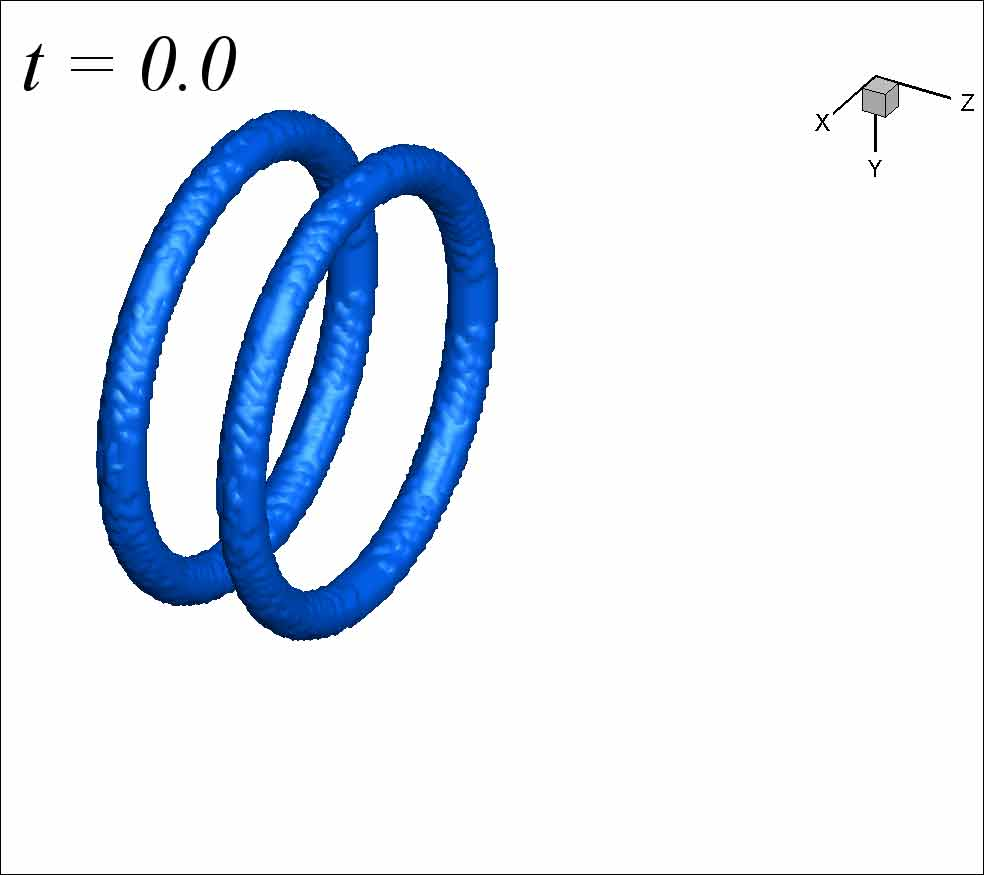
\includegraphics[width=0.65\linewidth]{figure1a.jpg}
\caption{Two pictures side by side with two captions (left)}\label{obraz2}
\end{minipage}
\quad
\begin{minipage}[t]{0.42\linewidth}
\centering
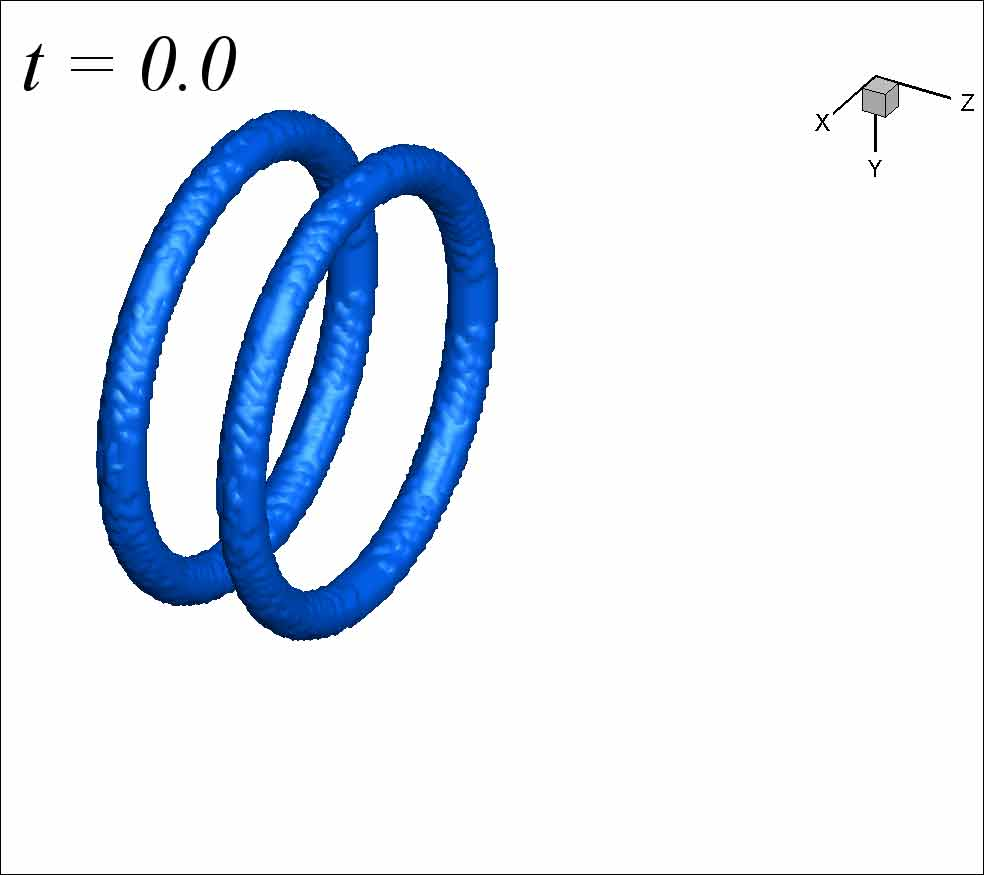
\includegraphics[width=0.65\linewidth]{figure1a.jpg}
\caption{Two pictures side by side with two captions (right)}\label{obraz3}
\end{minipage}
\end{figure}

Example of table is shown below (Tab. \ref{tab1} and Tab. \ref{tab:cryocoolers}).\\
\begin{table} [!ht]
\caption{Acceleration achieved for Jacobi's method.}\label{tab1}
\centerline{
\begin{tabular}{|c|c|c|c|c|}
\hline
Number of nodes & tsl  &  tx &  nc & frm nc\\
\hline
32x32x32 & 4.05 & 6.61 & 6.94 & 12.32\\
64x64x64 & 17.71 & 26.32 & 31.26 & 52.82\\
128x128x128 & 24.78 & 29.95 & 43.67 & 58.89\\
\hline
\end{tabular}}
\end{table}

Additional example of table is shown below.\\
\begin{table}[h]
    \centering
    \caption{Cryogenic coolers}
    \label{tab:cryocoolers}
    \begin{tabular}{@{}lll@{}}
    \toprule
    \begin{tabular}[c]{@{}c@{}}Cryooler\end{tabular} &
      \begin{tabular}[c]{@{}c@{}}Capacity range\end{tabular} &
      \multicolumn{1}{c}{ } \\ \midrule
    \begin{tabular}[c]{@{}c@{}}Turbo-Brayton\end{tabular}    & 18 - 250 kW at 120 K  \\
    \begin{tabular}[c]{@{}c@{}}Stirling\end{tabular}         & 2 - 8 kW at 120 K     \\
    \begin{tabular}[c]{@{}c@{}}Gifford-McMahon\end{tabular}  & 14 - 600 W at 80 K     \\
    \begin{tabular}[c]{@{}c@{}}2-stage Pulse Tube\end{tabular}  & up to 1.2 kW at 120 K  \\
    \begin{tabular}[c]{@{}c@{}}Single-stage Pulse Tube\end{tabular}  & 12 - 90 W at 80 K  \\
    \begin{tabular}[c]{@{}c@{}}Miniature Pulse Tube\end{tabular}       & 3 - 10 W at 80 K    \\
    \begin{tabular}[c]{@{}c@{}}Joule-Thomson\end{tabular}       & 100 W at 120 K   \\
    \begin{tabular}[c]{@{}c@{}}Cryogenic cascade\end{tabular}         & up to few kW at 120 K  \\ \bottomrule
    \end{tabular}
\end{table}

\begin{thebibliography}{1}
{\small %small is better for refs
\bibitem{Aref1} Aref H.  \textit{Motion of three vortices}, Phys. Fluids \textbf{22} (3), 393-400, 1997
\bibitem{Kochin} Kochin N. E.,  Kibel I. A., Roze N. V. \textit{Theoretical hydromechanics}, Interscience Publishers, New York 1965
\bibitem{Synge} Synge J. L. \textit{On the motion of three vortices}, Can. J. Math., \textbf{1}, 257-270, 1949
}
\end{thebibliography}

\end{document}
